\newpage

\section{Porównanie algorytmów detekcji oczu}



\subsection{Testowanie na statycznych zdjęciach}

Testowanie detekcji oczu wykorzystując statyczne zdjęcia odbywa się na obrazach z~przygotowanego zbioru (odrzucone~2, dla których wybrany algorytm nie wykrył prawidłowo twarzy). Znajduje się na nich w~sumie 166 oczu do wykrycia, w~tym~14 zamkniętych.

\subsubsection{Oczekiwany wynik}

Podobnie jak w~przypadku testowania detekcji twarzy na statycznych zdjęciach, tak również w~przypadku wykrywania oczu akceptowalny obszar został opisany dwoma prostokątami - minimalny i~maksymalnym. Przykład takiego oznaczenia widoczny jest na rysunku~\ref{fig:expected_eyes_region}. Oczekiwany obszar został dobrany w~następujący sposób:

\begin{itemize}
    \item prostokąt wewnętrzny obejmuje jedynie widoczną część gałki ocznej
    \item prostokąt zewnętrzny jest powiększony na boki i~w~dół o~pewną odległość od gałki, a~od góry zawiera w sobie również brwi.
\end{itemize}

\begin{figure}[!h]
    \begin{center}
        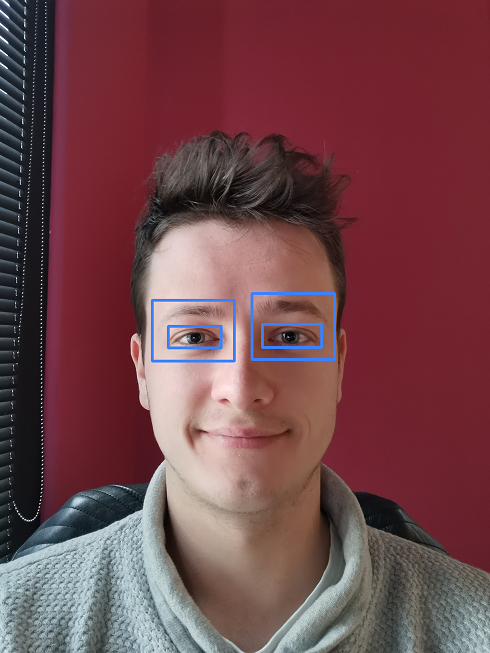
\includegraphics[scale=0.6]{img/eye_section/expected_eyes_region.png}
        \caption{Przybliżony obszar oczu, który jest oczekiwanym wynikiem algorytmu.}
        \label{fig:expected_eyes_region}
    \end{center}
\end{figure}

\subsubsection{Warunki testowania}

Oba algorytmy zostały przetestowane na wykrytych przez algorytm HOG twarzach ze~zdjęć~500x500. W~tym teście odrzucona została rozdzielczość~300x300, ze~względu, że~na części z~nich osoba jest już bardzo oddalona, co skutkuje bardzo małym rozmiarem oczu. W~przypadku korzystania z~przedniej kamery telefonu nie będą występowały takie odległości między twarzą, a~urządzeniem, żeby oczy zajmowały tak małą powierzchnię. Z~tego powodu takie warunki nie przyniosłyby znaczących i~wartościowych w~kontekście pracy dyplomowej wyników. 

\par

Testy zostały przeprowadzone w~przestrzeni barw RGB oraz w~skali szarości.

\subsubsection{Badanie skuteczności detekcji}

Na początku porównywana była skuteczność zaprezentowanych metod. Chociaż w~pewien sposób procent detekcji był już przedstawiony podczas dostrajania algorytmów, to tutaj zostały skonfrontowane ze~sobą oba algorytmy.

\par

W~przypadku metody opartej o~znaczniki twarzy, niewykryte oczy zarówno otwarte jak i~zamknięte mogą oznaczać źle określone położenie lub złą klasyfikacje do jednej z tych grup. Przykładowo oko otwarte mające EAR mniejszy niż ustalony próg klasyfikowane było jako zamknięte, co skutkowało oznaczeniem jako błędna detekcja. 

\begin{table}[!h]
\label{tab:eye_detection_accuracy_result}
\centering
\caption{Skuteczność algorytmów detekcji twarzy}
\resizebox{\textwidth}{!}{%
\begin{tabular}{|c|c|c|c|c|c|c|}
\hline
 &
  \textbf{\begin{tabular}[c]{@{}c@{}}Prawidłowe\\ detekcje\end{tabular}} &
  \textbf{\begin{tabular}[c]{@{}c@{}}Perfekcyjne\\ detekcje\end{tabular}} &
  \textbf{\begin{tabular}[c]{@{}c@{}}Częściowo\\ dobre\\ detekcje\end{tabular}} &
  \textbf{\begin{tabular}[c]{@{}c@{}}Złe\\ detekcje\end{tabular}} &
  \textbf{\begin{tabular}[c]{@{}c@{}}Niewykryte\\  oczy otwarte\end{tabular}}  &
 \textbf{\begin{tabular}[c]{@{}c@{}}Niewykryte\\  oczy zamknięte \end{tabular}} \\ \hline \hline

\textbf{Facemarki oczu RGB} &
  144 &
  142 &
  2 &
  12 &
  6 &
  6  \\ \hline
  
\textbf{\begin{tabular}[c]{@{}c@{}}Facemarki oczu \\ sk. szaro. \end{tabular}} &
  145 &
  140 &
  5 &
  11 &
  1 &
  6  \\ \hline
  
\textbf{Haar RGB} &
  133 &
  95 &
  38 &
  23 &
  9 &
  11  \\ \hline
  
\textbf{Haar sk. szaro.} &
  130 &
  95 &
  35 &
  26 &
  11 &
  7  \\ \hline
  
  \hline
\end{tabular}%
}
\end{table}

Najlepsze wyniki uzyskała metoda oparta na punktach charakterystycznych twarzy w~trójkanałowej przestrzeni barw. Udało się jej wykryć średnio $87\%$ wszystkich oczu, a~w~przypadku przestrzeni RGB aż~$86 \%$ z~nich perfekcyjnie. Ta druga statystyka jest dużo lepsza niż w~przypadku metody Haar, która uzyskała raptem~$57\%$. Algorytm wykorzystujący znaczniki był skuteczniejszy od drugiej metody o~około~$10\%$ jeśli weźmie się pod uwagę wykryte oczy. 

\par

Detekcja oczu przy pomocy znaczników i~EAR zwracała bardzo dobrze dopasowany rejon oczu, bez zbyt dużego narzutu w~postaci niepotrzebnych obszarów twarzy. Negatywne detekcje wynikały najczęściej ze zmrużonych oczu przez co współczynnik EAR sygnalizował, że~oczy są zamknięte. Jednak większość zwróconych obszarów była prawidłowa. Wyniki z~rozdziału~\ref{section:facemark_live_detection} sugerują również, że~w~ciężkich warunkach oświetleniowych detekcja oczu może nie dawać zadowalających wyników. Nie można zapominać o~fakcie, że~wpływ na skuteczność tej metody ma przede wszystkim dokładność odwzorowania znaczników wokół oczu. W~przypadku błędnej ich alokacji nie jest możliwe wykrycie prawidłowego obszaru oczu. 

\par

Największy problem klasyfikatorom kaskadowym używanym do wykrywania oczu sprawiły zdjęcia, na których osoba miała przekrzywioną pod kątem względem pionu głowę. Wynika to zapewne z samej natury algorytmu, ponieważ taki sam problem występował w~przypadku wykorzystania go do detekcji twarzy. Metoda Haar lepiej radziła sobie z~jasnym oświetleniem niż ta oparta na znacznikach. Cienie padające na obszar oczu również nie wpływały na obniżenie skuteczności detekcji. Miała ona problem z~wykryciem oczu w~przypadku gdy były one częściowo zasłonięte np.~włosami.Jeśli osoba na zdjęciu nosiła okulary to w~większości przypadków detekcja była na dobrym poziomie. Problem pojawiał się w~momencie gdy na szkłach występowały refleksy świetlne. Metodzie tej udało się prawidłowo wykryć większą liczbę przymkniętych oczu niż w~przypadku drugiej metody. Wynikało to z~faktu, że~klasyfikatory kaskadowe zwracała również lokalizację oczu całkowicie zamknięte. W~ramach projektu jest to skutek co najmniej niepożądany, z tego względu w~wynikach uznawany był za błędny. 



\vspace{5mm}

Ważną różnicą w~działaniu obu algorytmów jest kształt i~rozmiar oznaczanego obszaru. Metoda oparta o~klasyfikatory zwraca kwadratowy region, zawierający dużo większą część twarzy niż same oczy, np.~brwi. Natomiast punkty charakterystyczne tworzą obszar o~kształcie prostokąta o~dowolnym stosunku boków i~zawierają głównie samą gałkę oczną. Zmniejsza to ilość punktów, które mogą przeszkadzać w~innych aspektach analizy twarzy np.~podczas detekcji źrenic.

\vspace{5mm}

Porównując przestrzenie barw ciekawym wynikiem jest uzyskanie większej liczby dobrych detekcji przez metodę opartą o~znaczniki w przypadku obrazów w~skali szarości, ale mniej perfekcyjnych niż dla RGB. Natomiast, algorytm Haar lepiej poradził sobie w~przypadku trójkanałowego zestawu barw, ale wykrywał on więcej zamkniętych oczu jako otwarte przez co w~tej statystyce wypadł gorzej niż w skali szarości. 




\subsubsection{Badanie szybkości detekcji} \label{section:eye_detection_speed_img}

Dla detekcji oczu z~użyciem znaczników twarzy zostały przedstawione dwa wyniki czasowe - jeden uwzględniający czas wykrycia punktów charakterystycznych, a~drugi bez. Związane jest to z~faktem, że~mimo iż do wykorzystania tej metody niezbędna jest detekcja facemarków, to etap taki i~tak będzie wykonany, ponieważ punkty te są używane np.~do stwierdzenia mrugnięcia. 

\par 

W~przypadku czasów zawierających algorytm wykrywania punktów charakterystycznych test był przeprowadzony dla dwóch przestrzeni barw. Natomiast, na szybkość przekształcenia facemarków w~obszar oka nie wpływa liczba kanałów, ponieważ nie operuje on na pikselach, tylko na zwróconych punktach kartezjańskich. Z~tego powodu przedstawiony jest tylko jeden wynik.

\vspace{4mm}

\begin{table}[!h]
\label{tab:eye_detect_speed_RGB}
\centering
\caption{Czas przetwarzania algorytmów detekcji twarzy dla obrazów RGB}

\begin{tabular}{|c|c|c|c|}
\hline
 & 
  \textbf{\begin{tabular}[c]{@{}c@{}}Całkowity czas \\ przetwarzania \end{tabular}} &
  \textbf{\begin{tabular}[c]{@{}c@{}}Średni czas\\ przetwarzania \\ pojedynczej iteracji\end{tabular}} &
  \textbf{\begin{tabular}[c]{@{}c@{}}Średni czas\\przetwarzania \\ pojedynczego\\zdjęcia\end{tabular}} \\ \hline\hline
  
\textbf{\begin{tabular}[c]{@{}c@{}}Facemarki oczu RGB\\ (z detekcją facemarków)\end{tabular}} & 
  5,638 s &
  0,281 s &
  0,00361 s    \\ \hline
  
  \textbf{\begin{tabular}[c]{@{}c@{}}Facemarki oczu sk. szaro. \\ (z detekcją facemarków)\end{tabular}} & 
  5,803 s &
  0,290 s &
  0,00372 s    \\ \hline
  
\textbf{\begin{tabular}[c]{@{}c@{}}Facemarki oczu \\ (bez detekcją facemarków)\end{tabular}} & 
  0,024 s &
  0,00122 s &
  0,00000157 s  \\ \hline
  
\textbf{Haar RGB} & 
  26,219 s &
  1,310 s &
  0,0168 s     \\ \hline
  
\textbf{Haar sk. szaro.} & 
  25,830 s &
  1,291 s &
  0,0165 s    \\ \hline
  
  \hline
\end{tabular}%

\end{table}

\par

Wyniki bezdyskusyjnie pokazują dużo większą szybkość detekcji oczu z~użyciem znaczników. Nawet biorąc pod uwagę czas wykrycia punktów charakterystycznych metoda ta była ponad~$4$ razy szybsza od algorytmu opartego na klasyfikatorach kaskadowych Haar. 

\par

Tworzenie obszarów ze~znaczników osiągnęło czas rzędu~$10^{-5}s$, co~w~porównaniu do pozostałych algorytmów wykorzystywanych w projekcie jest praktycznie natychmiastowe. Tak bliski zeru czas przetwarzania sprawia, że~nie ma on żadnego wpływu na ilość klatek na sekundę podczas odbierania obrazu na żywo z~kamery.

\par

Przestrzeń barw nie miała znaczącego wpływu na czas detekcji, a~wyniki w~przypadku trójkanałowych kolorów były porównywalne do skali szarości.




\subsection{Testowanie na obrazie z~kamery na żywo}

Detekcja oczu została przetestowana również na obrazie z~kamery na żywo. Warunki przeprowadzenia eksperymentu zostały opisane w~rozdziale~\hyperref[{section:face_detection_test_live}]{\ref{section:face_detection_test_live}}.

\subsubsection{Badanie skuteczność detekcji}

Obserwując na żywo detekcje oczu autor projektu był w~stanie wysnuć kilka wniosków na temat badanych algorytmów.

\vspace{4mm}

Przede wszystkim oba działały bardzo stabilnie. Nie występowało nieuzasadnione gubienie obszaru oczu podczas statycznego położenia głowy i urządzenia. W~metodzie Haar występował problem przy mocnym skręceniu głowy w~bok. Zwracany był wtedy często błędny i~bardzo powiększony obszar dalszego oka. Natomiast detekcja oczu na podstawie znaczników miała problemu z~mocno przymkniętymi oczami. Wskaźnik EAR sygnalizował wtedy je jako zamknięte przez co algorytm nie zwracał ich regionu.

\par

Subiektywnie oceniając obie metody dają zadowalające i~wystarczające rezultaty z~perspektywy pracy dyplomowej, ale ze względu na stabilniejsze działanie metody wykorzystującej znaczniki podczas ruchów głową uznany został za lepsze rozwiązanie w~tym przypadku.


\subsubsection{Badanie szybkość detekcji} \label{section:eye_speed_live}

Ze względu na praktycznie zerowy obciążenie podczas przekształcania znaczników w~obszar twarzy (rozdz.~\hyperref[{section:eye_detection_speed_img}]{\ref{section:eye_detection_speed_img}}), wyniki dla facemarków zostały skopiowane z~rezultatów uzyskanych przez algorytm Kazemi podczas porównania metod nakładania punktów charakterystycznych na obraz z~kamery na żywo w~rozdziale~\hyperref[{section:facemark_speed_live}]{\ref{section:facemark_speed_live}}.

\par

Ponownie detekcja twarzy odbywała się przy zastosowaniu algorytmu HOG dostarczając obraz RGB.

\begin{table}[!h]
\label{tab:eye_detection_speed_live}
\centering
\caption{Szybkość algorytmów detekcji oczu dla obrazu na żywo z kamery [klatki/s]}
\begin{tabular}{|c|c|c|c|c|c|}
\hline
 \textbf{\begin{tabular}[c]{@{}c@{}}Warunki\end{tabular}} &
  \begin{tabular}[c]{@{}c@{}}1.\end{tabular} &
  \begin{tabular}[c]{@{}c@{}}2.\end{tabular} &
  \begin{tabular}[c]{@{}c@{}}3.\end{tabular} &
  \begin{tabular}[c]{@{}c@{}}4.\end{tabular} &
  \textbf{\begin{tabular}[c]{@{}c@{}}Średnia:\end{tabular}}\\ \hline \hline
\textbf{Haar RGB} &
  11,698 &
  13,600 &
  12,290 &
  12,942 &
  12,632  \\ \hline

\textbf{Haar sk. szaro.} &
  11,956 &
  12,403 &
  12,333 &
  12,472 &
  12,290 \\ \hline
  
\textbf{Znaczniki RGB} &
  15,887 &
  15,941 &
  16,077 &
  16,171 &
  16,019  \\ \hline
  
\textbf{Znaczniki sk. szaro.} &
  15,747 &
  16,146 &
  15,866 &
  16,096 &
  15,963 \\ \hline

  \hline
\end{tabular}%

\end{table}

Wyniki przeprowadzonych badań przedstawiają znaczną przewagę szybkościową metody opartej na znacznikach. Klasyfikatory kaskadowe uzyskały około~$23\%$ mniejszą liczbę klatek na sekundę, co jest znaczącym obniżeniem wydajności.



\subsection{Wybór algorytmu detekcji oczu}

Porównanie dwóch algorytmów detekcji oczu bezdyskusyjnie pokazało wyższość metody opartej na znacznikach nad klasyfikatorem kaskadowym Haar. Punkty charakterystyczne uzyskały lepszy procentowo wynik prawidłowych detekcji, a~dodatkowo w~teście na statycznych zdjęciach prawie wszystkie były perfekcyjne. Próby szybkościowe jednoznacznie wskazały na znaczniki, które były $4$ razy szybsze od Haar, a~jeśli brać pod uwagę jedynie czas tworzenia obszarów to ponad tysiąckrotnie i~ich przetwarzanie jest niezauważalne z~perspektywy pozostałych detekcji.

\vspace{5mm}

Na podstawie przeprowadzonych testów znaczniki twarzy zostały wybrane do detekcji oczu i~to ten algorytm jest wykorzystywany w~projekcie i~pracy dyplomowej.